
\chapter{Αλγόριθμοι μείωσης διαστάσεων}
\numberwithin{equation}{section}

\section{Γραμμική μείωση διαστάσεων}
\par
Όλες οι τεχνικές μείωσης διαστάσεων στις οποίες έχουμε αναφερθεί μέχρι στιγμής είναι κατεξοχήν τεχνικές μείωσης της διάστασης του χώρου των χαρακτηριστικών. Μάλιστα το ιδιαίτερο χαρακτηριστικό τους είναι ότι αποτελούν μεθόδους οι οποίες σέβονται την γραμμικότητα. Η μέθοδος \textlatin{PCA} για παράδειγμα η οποία αποτελεί μια απο τις γνωστότερες αλλά και πιο ισχυρές μεθόδους γραμμικής μείωσης διαστάσεων λειτουργεί καλά αν τα σημεία των δεδομένων είναι κατανεμημένα σε ένα υπερεπίπεδο. Όπως αναλύθηκε στην ενότητα (2.2) η μέθοδος \textlatin{PCA} προβάλλει στις διευθύνσεις μέγιστης διασποράς. Επίσης όπως εξηγήσαμε στο προηγούμενο κεφάλαιο η ανάλυση ιδιοτιμών-ιδιοδιανυσμάτων του μητρώου συσχέτισης αποκαλύπτει την διάσταση του υπερεπιπέδου στο οποίο τα δεδομένα είναι διεσπαρμένα. 
\par
Με άλλα λόγια δηλαδή η διάσταση είναι ένα μέτρο του πλήθους των ελεύθερων μεταβλητών που είναι υπεύθυνες για τον τρόπο με τον οποίο μεταβάλλεται ένα σήμα, δηλαδή για την πραγματική πληροφορία την οποία κωδικοποιούν τα δεδομένα. 
\par
Παρότι ο αλγόριθμος \textlatin{PCA} αποτελεί μία πολύ ισχυρή και ευρέως χρησιμοποιούμενη μέθοδο μείωσης της διάστασης υπάρχουν περιπτώσεις στις οποίες η μέθοδος αποτυγχάνει. Τέτοιες είναι περιπτώσεις κατα τις οποίες ο μηχανισμός παραγωγής των δεδομένων είναι έντονα μη γραμμικός με αποτέλεσμα τα δεδομένα να κείτονται σε πιο περίπλοκες πολλαπλότητες. Ας πάρουμε για παράδειγμα τις εξισώσεις \\
\begin{center}
$x_{1}=r cos\theta, \quad x_{2}=rsin\theta$
\end{center}
Προφανώς απο τις παραπάνω εξισώσεις είναι φανερό ότι το $x$ βρίσκεται στην περιφέρεια κύκλου ακτίνας $r$. Πρόκειται δηλαδή για πρόβλημα μονοδιάστατης πολλαπλότητας αφού αρκεί μια μόνο μεταβλητή για την περιγραφή των δεδομένων. Η παράμετρος αυτή είναι η απόσταση κατα μήκος της περιφέρειας απο ένα σημείο(αφετηρία) πάνω στην περίμετρο του κύκλου. Αν λοιπόν εφαρμόσουμε την μέθοδο \textlatin{PCA} στο παραπάνω σύνολο δεδομένων τότε η απάντηση που θα μας δώσει για την διάσταση των δεδομένων θα είναι, λανθασμένα προφανώς, ίση με δύο. 
\par
Περιπτώσεις όπως οι παραπάνω απαιτούν αλγορίθμους μείωσης διάστασης και εξαγωγής χαρακτηριστικών οι οποίοι να λαμβάνουν υπόψιν την γεωμετρία του προβλήματος ώστε να μπορούν να εξάγουν ασφαλή συμπεράσματα για την διάσταση των δεδομένων. Στον τομέα της υπολογιστικής όρασης για παράδειγμα, ο οποίος όπως αναφέραμε και παραπάνω αποτελεί βασικό κομμάτι της εν λόγω διατριβής, απαιτούνται κατεξοχήν αλγόριθμοι μη γραμμικής μείωσης διαστάσεων αφού οι εικόνες ή τα χαρακτηριστκά των εικόνων τα οποία αποτελούν τα δεδομένα μας είναι κατα κύριο λόγο μη γραμμικά. 

\section{Μη γραμμική μείωση διαστάσεων}
\par
Υπάρχει λοιπόν μια ευρεία γκάμα εφαρμογών οι οποίες απαιτούν αλγορίθμους μη γραμμικής μείωσης διαστάσεων. Αυτό συμβαίνει διότι στις συγκεκριμένες εφαρμογές η γεωμετρική αναπαράσταση των δεδομένων είναι τέτοια ώστε απαιτείται να βρεθεί μια ενσωμάτωση μικρότερης διάστασης η οποία βρίσκεται <<κρυμμένη>> στον χώρο των αρχικών διαστάσεων. Θα πρέπει μάλιστα κατά την διαδικασία αυτή να ληφθούν υπόψιν τα γεωμετρικά χαρακτηριστικά του χώρου των δεδομένων. 
\par
Έχει πολύ μεγάλη σημασία στο σημείο αυτό να κατανοήσουμε τι εννοούμε όταν αναφερόμαστε στα γεωμετρικά χαρακτηριστικά του προβλήματος. Το πιο χαρακτηριστικό και ευρέως χρησιμοποιούμενο παράδειγμα για τον σκοπό αυτό είναι ένα τεχνητό σετ δεδομένων, με την όνομασία \textlatin{Swiss Roll} το οποίο φαίνεται στην παρακάτω εικόνα. \\
\vspace{1.0cm}
\begin{figure}[h]
\centering
%\hspace*{2.5cm}
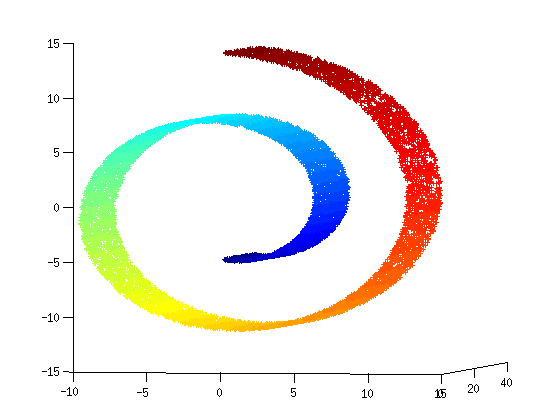
\includegraphics[scale=0.8]{figs/2.png}
\newline
\caption{ \textlatin{Swiss Roll Synthetic Dataset}.} 
\end{figure}
\vspace{1.0cm}
\par
Αυτό που αξίζει να παρατηρηθεί λοιπόν στο παραπάνω σετ δεδομένων είναι ότι αν για παράδειγμα διαλέξουμε κάποιο οποιοδήποτε σημείο του απο την κόκκινη περιοχή και προσπαθήσουμε να βρούμε ποιά δεδομένα αποτελούν κοντινότερους γείτονες του σημείου αυτού πιθανότατα θα πέφταμε στην παγίδα, όπως και οι τεχνικές γραμμικής μείωσης διαστάσεων, να πούμε ότι κάποια σημεία απο την μπλέ περιοχή βρίσκονται και αυτά στην γειτονιά του σημείου που διαλέξαμε. Αυτό προφανώς είναι λάθος αφού απο τον χρωματισμό των παραπάνω δεδομένων αντιλαμβανόμαστε ότι στην πραγματικότητα τα μπλέ δεδομένα βρίσκονται πολύ μακριά απο τα κόκκινα. Ο παραπάνω εσφαλμένος συλλογισμός αναπαρίσταται στο παρακάτω γράφημα.
\par
\begin{figure}[h!]
\centering
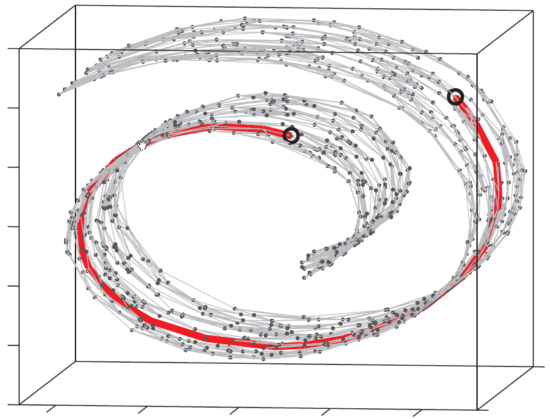
\includegraphics[scale=0.5]{figs/3.png}
\newline
\caption{\textlatin{Swiss Roll Synthetic Dataset Manifold Learning Path.}} 
\end{figure}
\par
\vspace*{2cm}
Αντιλαμβανόμαστε λοιπόν, μέσω της παραπάνω απεικόνισης ότι θα πρέπει να ληφθεί υπόψιν η γεωμετρία του προβλήματος ώστε σε καμιά περίπτωση υπολογίζοντας κοντινότερες αποστάσεις να συμπεριλάβουμε το αρχικό και το τελικό σημείο ως κοντινούς γείτονες, ενώντάς τα απευθείας μεταξύ τους. Αυτή είναι και η διαφορά των αλγορίθμων μη γραμμικής μείωσης διαστάσεων με αυτούς της γραμμικής. Για να γίνει πλήρως κατανοητός ο τρόπος μείωσης των διαστάσεων του παραπάνω σετ δεδομένων, δίνεται η απεικόνιση των δεδομένων σε χώρο χαμηλής διάστασης μετά απο την εφαρμογή αλγορίθμου μη γραμμικής μείωσης διαστάσεων.
\clearpage
\begin{figure}[t]
\centering
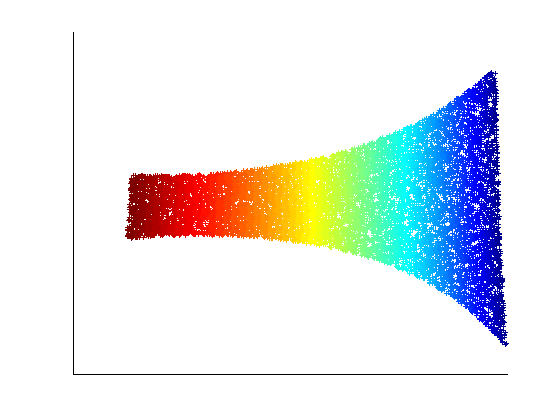
\includegraphics[scale=0.8]{figs/4.png}
\newline
\caption{\textlatin{Dimensionality Reduction with LLE (K=16,d=2).}} 
\end{figure}
\par
\vspace*{1cm}
Απο την παραπάνω απεικόνιση μπορούμε να συμπεράνουμε ότι κάνοντας μείωση των διαστάσεων στην πραγματικότητα <<ξετυλίξαμε>> το \textlatin{Swiss Roll} και έτσι απο τον αρχικό χώρο των τριών διαστάσεων στην πραγματικότητα η εγγενής διάσταση των δεδομένων είναι ίση με δύο. Στις επόμενες ενότητες θα γίνει παρουσίαση των πιο γνωστών μεθόδων μη γραμμικής μείωσης διαστάσεων καθώς επίσης θα γίνει και η μαθηματική τους ανάλυση.


\subsection{\textlatin{ISOMAP}}
\par
Ένας βασικός αλγόριθμος μη γραμμικής μείωσης διαστάσεων είναι ο αλγόριθμος Ισομετρική απεικόνιση \textlatin{(Isometric Mapping - ISOMAP)}\textlatin{\cite{isomap}}. Ο αλγόριθμος αυτός υιοθετεί την άποψη ότι μόνο οι γεωδαιτικές αποστάσεις μεταξύ όλων των ζευγών των σημείων των δεδομένων μπορούν να αντικατοπτρίσουν την πραγματική δομή της πολλαπλότητας του προβλήματος. Η παραπάνω διατύπωση αντικατοπτρίζει το παράδειγμα που δόθηκε στο γράφημα (3.2), και τονίζει το γεγονός ότι οι Ευκλείδιες αποστάσεις μεταξύ σημείων μιας πολλαπλότητας δεν μπορούν να την αναπαραστήσουν ικανοποιητικά. Αυτό διότι σημεία (στο γράφημα τα δύο σημεία που έχουν επισυμανθεί με μαύρους κύκλους) που είναι απομακρυσμένα μεταξύ τους σύμφωνα με την γεωδαιτική απόσταση, μπορεί να θεωρηθούν λανθασμένα, κοντικά ως προς την Ευκλείδια απόστασή τους.
\par
Ουσιαστικά η μέθοδος \href{http://isomap.stanford.edu/}{\textlatin{ISOMAP}} είναι μια παραλλαγή του αλγορίθμου \href{https://en.wikipedia.org/wiki/Multidimensional_scaling}{\textlatin{Multi Dimensional Scaling - MDS}}, με την διαφορά ότι οι Ευκλείδιες αποστάσεις αντικαθίστανται απο τις αντίστοιχες γεωδαιτικές κατά μήκος της πολλαπλότητας των δεδομένων. Η ουσία του αλγορίθμου είναι να εκτιμηθούν σωστά οι γεωδαιτικές αποστάσεις μεταξύ σημείων τα οποία είναι απομακρυσμένα μεταξύ τους. Ο αλγόριθμος μπορεί να χωριστεί σε δύο βασικά βήματα:
\par
\textbf{Βήμα-1}: \\ Για κάθε σημείο $x_{i},i=1,1\ldots,n$, υπολόγισε τους πλησιέστερους γείτονες και κατασκέυασε έναν γράφο $G(V,E)$ του οποίου οι κορυφές αναπαριστούν πρότυπα εισόδου και οι ακμές συνδέουν τους πλησιέστερους γείτονες. Οι παράμετροι $k$ (αριθμός των κοντινών γειτόνων κάθε σημείου) ή $\epsilon$ (ακτίνα σφαίρας στην οποία ανήκουν γειτονικά σημεία) είναι παράμετροι που καθορίζονται απο τον χρήστη. Στις ακμές ανατίθενται βάρη σύμφωνα με τις αντίστοιχες Ευκλείδιες αποστάσεις (για τους πλησιέστερους γείτονες αυτή είναι μια καλή προσέγγιση της γεωδαιτικής απόστασης).
\par
\textbf{Βήμα-2}: \\ Υπολόγισε ανα ζεύγος την γεωδαιτική απόσταση για όλα τα ζεύγη κατα μήκος των συντομότερων διαδρομών μέσα στον γράφο. Το πιο σημαντικό σημείο, είναι ότι η γεωδαιτική απόσταση μεταξύ δύο οποιονδήποτε σημείων της πολλαπλότητας μπορεί να προσεγγιστεί μέσω της συντομότερης διαδρομής που ενώνει τα δύο σημείο στο γράφο $G(V,E)$. Ο πιο γνωστός αλγόριθμος υλοποίησης της παραπάνω διαδικασίας είναι ο αλγόριθμος \textlatin{Djikstar} με πολυπλοκότητα $\mathcal{O}(n^{2}\ln n + n^{2}k)$, μέγεθος απαγορευτικό για τις περισσότερες πρακτικές εφαρμογές.
\par
Εφόσον έχουν εκτελεστεί τα δύο αυτά βήματα είμαστε πλέον σε θέση νε εφαρμόσουμε την κλασική μέθοδο \textlatin{MDS}. Το πρόβλημα λοιπόν απο εδώ και στο εξής γίνεται ισοδύναμο με την εφαρμογή της ανάλυσης ιδιοδιανυσμάτων του αντίστοιχου μητρώου \textlatin{Gram} και την επιλογή των \textlatin{m} περισσότερο σημαντικών ιδιοδιανυσμάτων για την αναπαράσταση του χώρου χαμηλής διάστασης. Μετά απο αυτή την αναπαράσταση, οι Ευκλείδιες αποστάσεις μεταξύ των σημείων του χώρου χαμηλής διάστασης ταιριάζουν με τις αντίστοιχες γεωδαιτικές αποστάσεις στην πολλαπλότητα του αρχικού χώρου υψηλής διάστασης. Όπως και στις μεθόδους \textlatin{PCA} και \textlatin{MDS} η διάσταση \textlatin{m} εκτιμάται απο το πλήθος των \textlatin{m} περισσότερο σημαντικών ιδιοτιμών. Αποδεικνύεται τέλος ότι η μέθοδος \textlatin{ISOMAP} ασυμπτωτικά ($n \rightarrow \inf$) θα ανακτήσει την αληθινή διάσταση για ένα σύνολο δεδομένων μη γραμμικής πολλαπλότητας.

\subsection{\textlatin{Laplassian Eigenmaps}}
\par
Η μέθοδος αυτή \textlatin{\cite{laplassianeigenmaps}} στηρίζεται στην υπόθεση ότι τα σημεία των δεδομένων βρίσκονται σε μια λεία πολλαπλότητα $ Μ \supset Χ $, της οποίας η εγγενής διάσταση είναι ίση με $m<N$ και είναι ενσωματωμένη στον $ \Re^{N} $, δηλαδή $ Μ \supset \Re^{N} $. Η διάσταση $m$ δίνεται ως παράμετρος απο τον χρήστη και εξαρτάται απο το σύνολο των δεδομένων για κάθε εφαρμογή. Η κύρια φιλοσοφία πίσω απο την μέθοδο είναι να υπολογιστεί η αναπαράσταση των δεδομένων σε χώρο χαμηλής διάστασης, έτσι ώστε η τοπική πληροφορία γειτνίασης στον χώρο $Χ \supset M$ να διατηρείται κατά βέλτιστο τρόπο. Με τον τρόπο αυτό προσπαθούμε να βρούμε μια λύση που αντανακλά τη γεωμετρική δομή της πολλαπλότητας. Για την επίτευξη αυτού απαιτούνται τα παρακάτω βήματα:
\par
\textbf{Βήμα-1}: Κατασκευή ενός γράφου $G=(V,E)$, όπου $V={v_{i},i=1,2,\ldots,n}$ είναι ένα σύνολο κορυφών και $E={\epsilon_{ij}}$ το σύνολο των ακμών που συνδέουν κορυφές $(v_{i},v_{j})$. Κάθε κόμβος $v_{i}$ του γράφου αντιστοιχεί σε ένα σημείο $\mathbf{x}_{i}$ του συνόλου των δεδομένων $X$. Συνδέουμε τις $v_{i}$,$v_{j}$, δηλαδή εισάγουμε την ακμή $\epsilon_{ij}$ μεταξύ των αντίστοιχων κόμβων, αν τα σημεία $\mathbf{x}_{i},\mathbf{x}_{j}$ είναι μεταξύ τους κοντινά. Η μέθοδος ορίζει την εγγύτητα αυτή με δύο τρόπους: \\
1. $\Vert \mathbf{x}_{i}-\mathbf{x}_{j} \Vert ^{2} < \epsilon $, για κάποια παράμετρο $\epsilon$ η οποία ορίζεται απο τον χρήστη. Με $\Vert\cdot\Vert$ ορίζουμε την πράξη της Ευκλείδιας νόρμας στον χώρο $\Re^{N}$. \\
2. Το $\mathbf{x}_{j}$ είναι μεταξύ των $k$ πλησιέστερων γειτόνων του $\mathbf{x}_{i}$ ή και αντίστροφα, με το $k$ να είναι και σε αυτή την περίπτωση είσοδος η οποία καθορίζεται απο τον χρήστη. Επίσης οι γείτονες επιλέγονται χρησιμοποιώντας την μετρική της Ευκλείδιας απόστασης στον χώρο $\Re^{N}$. Η χρήση της Ευκλείδιας απόστασης αιτιολογείται απο την υπόθεση ότι η πολλαπλότητα είναι λεία, γεγονός που μας επιτρέπει να προσεγγίσουμε, τοπικά, τη γεωδαισία της πολλαπλότητας με Ευκλείδιες αποστάσεις.
\par
Για να αποσαφηνιστεί πλήρως η παραπάνω διατύπωση δίνεται το χαρακτηριστικό παράδειγμα όπου θεωρούμε μια σφαίρα ενσωματωμένη στον τρισδιάστατο χώρο, και έστω κάποιος περιορίζεται να ζεί πάνω στην επιφάνεια της σφαίρας. Τότε η συντομότερη διαδρομή απο ένα σημείο της σφαίρας σε ένα άλλο είναι η γεωδαιτική διαδρομή μεταξύ των δύο σημείων. Προφανώς αυτή δεν θα είναι ευθεία γραμμή, αλλά ένα τόξο στην επιφάνεια της σφαίρας. Παρ'όλα αυτά όμως, αν τα δύο σημεία είναι πολύ κοντά μεταξύ τους, η γεωδαιτική απόσταση μπορεί να προσεγγιστεί απο την Ευκλείδια απόσταση, υπολογισμένη στον τρισδιάστατο χώρο.
\par
\textbf{Βήμα-2}: Κάθε ακμή $\epsilon_{ij}$ συσχετίζεται με ένα βάρος $W(i,j)$. Για κόμβους που δεν συνδέονται μεταξύ τους, τα αντίστοιχα βάρη είναι μηδέν. Κάθε βάρος $W(i,j)$ είναι ένα μέτρο της εγγύτητας των αντίστοιχων γειτόνων $\mathbf{x}_{i},\mathbf{x}_{j}$. Μια τυπική επιλογή είναι \\
\newline\hspace*{\fill}
\[W(i,j) = \begin{cases} \exp(\Vert \frac{\mathbf{x}_{i}-\mathbf{x}_{j}}{\sigma^{2}} \Vert) \quad ,if \quad x_{i},x_{j} \quad neighbors\\
               0  \quad \quad \quad \quad \quad \quad ,not \quad neighbors\\
            \end{cases} \]
\hspace*{\fill}\newline 
με $\sigma^{2}$, παράμετρος η οποία ορίζεται και αυτή απο τον χρήστη. Σχηματίζουμε το μητρώο βαρών $W$, μεγέθους ($n \times n$), το οποίο έχει για στοιχεία τα βάρη $W(i,j)$. Σημειώνουμε ότι το $W$ είναι συμμετρικό και αραιό αφού στην πράξη προκύπτει ότι πολλά απο τα στοιχεία του είναι μηδενικά.
\par
\textbf{Βήμα-3}: Ορίζεται το διαγώνιο μητρώο $D$ με στοιχεία $D_{ij}=\sum_{j} W(i,j),i=1,2,\ldots,n,$ καθώς και το μητρώο $L=D-W$. Το τελευταίο είναι γνωστό ως το μητρώο \textlatin{Laplace} του γράφου $G=(V,E)$. Εφαρμόζεται η γενικευμένη ανάλυση σε ιδιοτιμές και ιδιοδιανύσματα 
\newline\hspace*{\fill}
$ \Lambda \mathbf{v} =  \lambda D \mathbf{v} $
\hspace*{\fill}\newline 
Έστω $ 0 = \lambda_{0} \leq \lambda_{1} \leq \lambda_{2} \leq \ldots \leq \lambda_{m}$, οι $m+1$ μικρότερες ιδιοτιμές. Αγνοείται η ιδιοτιμή $\mathbf{v}_{0}$ που αντιστοιχεί στην ιδιοτιμή $\lambda_{0} = 0$ και επιλέγονται τα υπόλοιπα $m$ ιδιοδιανύσματα $\mathbf{v}_{1},\mathbf{v}_{2},\ldots,\mathbf{v}_{m},$. Στην συνέχεια εκτελείται η απεικόνιση
\newline\hspace*{\fill}
$\mathbf{x}_{i} \in \Re^{N} \mapsto \mathbf{y}_{i} \in \Re^{m}, i=1,2,\ldots,n$
\hspace*{\fill}\newline 
όπου 
\newline\hspace*{\fill}
$\mathbf{y}_{i}^{T} = [\mathbf{v}_{1}(i),\mathbf{v}_{2}(i),\ldots,\mathbf{v}_{m}(i)], i=1,2,\ldots,m$
\hspace*{\fill}\newline
\par
Όπως έχουμε αναλύσει στην αντίστοιχη εντότητα η πολυπλοκότητα υπολογισμού ιδιοτιμών και ιδιοδιανυσμάτων είναι, γενικά, της τάξης $\mathcal{O}(n^{3})$. Ωστόσο για αραιά μητρώα, όπως στην συγκεκριμένη περίπτωση το $L$, μπορούν να εφαρμοστούν αποτελεσματικές τεχνικές με αποτέλεσμα την μείωση της πολυπλοκότητας σε τάξη κάποιο πολλαπλάσιο του $\mathcal{O}(n^2)$. Η πιο γνωστή και αποτελεσματική τεχνική για τον σκοπό αυτό είναι ο αλγόριθμος \textlatin{Lanczos}\textlatin{\cite{lanczos}}.
\par
Ο αλγόριθμος \textlatin{Laplassian Eigenmaps} ο οποίος αναλύθηκε παραπάνω, ανήκει στην ίδια κατηγορία (\textit{μέθοδοι μείωσης διαστάσεων που βασίζονται σε γράφους}) με τον αλγόριθμο \textbf{\textlatin{Locally Linear Embeddings - LLE}} ο οποίος αποτελεί και βασικό αντικείμενο της εν λόγω διατριβής. Οι δύο αλγόριθμοι έχουν πολύ κοινή λογική και μεθοδολογία και γι αυτό στο επόμενο κεφάλαιο στο οποίο γίνεται αναλυτική μαθηματική ανάλυση του \textlatin{LLE} θα αποσαφηνιστούν και τα παραπάνω βήματα του \textlatin{Laplassian Eigenmaps} καθώς τα βήματα τους είναι πανομοιότυπα.

